% Options for packages loaded elsewhere
% Options for packages loaded elsewhere
\PassOptionsToPackage{unicode}{hyperref}
\PassOptionsToPackage{hyphens}{url}
\PassOptionsToPackage{dvipsnames,svgnames,x11names}{xcolor}
%
\documentclass[
  english,
  letterpaper,
  DIV=11,
  numbers=noendperiod]{scrreprt}
\usepackage{xcolor}
\usepackage{amsmath,amssymb}
\setcounter{secnumdepth}{5}
\usepackage{iftex}
\ifPDFTeX
  \usepackage[T1]{fontenc}
  \usepackage[utf8]{inputenc}
  \usepackage{textcomp} % provide euro and other symbols
\else % if luatex or xetex
  \usepackage{unicode-math} % this also loads fontspec
  \defaultfontfeatures{Scale=MatchLowercase}
  \defaultfontfeatures[\rmfamily]{Ligatures=TeX,Scale=1}
\fi
\usepackage{lmodern}
\ifPDFTeX\else
  % xetex/luatex font selection
\fi
% Use upquote if available, for straight quotes in verbatim environments
\IfFileExists{upquote.sty}{\usepackage{upquote}}{}
\IfFileExists{microtype.sty}{% use microtype if available
  \usepackage[]{microtype}
  \UseMicrotypeSet[protrusion]{basicmath} % disable protrusion for tt fonts
}{}
\makeatletter
\@ifundefined{KOMAClassName}{% if non-KOMA class
  \IfFileExists{parskip.sty}{%
    \usepackage{parskip}
  }{% else
    \setlength{\parindent}{0pt}
    \setlength{\parskip}{6pt plus 2pt minus 1pt}}
}{% if KOMA class
  \KOMAoptions{parskip=half}}
\makeatother
% Make \paragraph and \subparagraph free-standing
\makeatletter
\ifx\paragraph\undefined\else
  \let\oldparagraph\paragraph
  \renewcommand{\paragraph}{
    \@ifstar
      \xxxParagraphStar
      \xxxParagraphNoStar
  }
  \newcommand{\xxxParagraphStar}[1]{\oldparagraph*{#1}\mbox{}}
  \newcommand{\xxxParagraphNoStar}[1]{\oldparagraph{#1}\mbox{}}
\fi
\ifx\subparagraph\undefined\else
  \let\oldsubparagraph\subparagraph
  \renewcommand{\subparagraph}{
    \@ifstar
      \xxxSubParagraphStar
      \xxxSubParagraphNoStar
  }
  \newcommand{\xxxSubParagraphStar}[1]{\oldsubparagraph*{#1}\mbox{}}
  \newcommand{\xxxSubParagraphNoStar}[1]{\oldsubparagraph{#1}\mbox{}}
\fi
\makeatother

\usepackage{color}
\usepackage{fancyvrb}
\newcommand{\VerbBar}{|}
\newcommand{\VERB}{\Verb[commandchars=\\\{\}]}
\DefineVerbatimEnvironment{Highlighting}{Verbatim}{commandchars=\\\{\}}
% Add ',fontsize=\small' for more characters per line
\usepackage{framed}
\definecolor{shadecolor}{RGB}{241,243,245}
\newenvironment{Shaded}{\begin{snugshade}}{\end{snugshade}}
\newcommand{\AlertTok}[1]{\textcolor[rgb]{0.68,0.00,0.00}{#1}}
\newcommand{\AnnotationTok}[1]{\textcolor[rgb]{0.37,0.37,0.37}{#1}}
\newcommand{\AttributeTok}[1]{\textcolor[rgb]{0.40,0.45,0.13}{#1}}
\newcommand{\BaseNTok}[1]{\textcolor[rgb]{0.68,0.00,0.00}{#1}}
\newcommand{\BuiltInTok}[1]{\textcolor[rgb]{0.00,0.23,0.31}{#1}}
\newcommand{\CharTok}[1]{\textcolor[rgb]{0.13,0.47,0.30}{#1}}
\newcommand{\CommentTok}[1]{\textcolor[rgb]{0.37,0.37,0.37}{#1}}
\newcommand{\CommentVarTok}[1]{\textcolor[rgb]{0.37,0.37,0.37}{\textit{#1}}}
\newcommand{\ConstantTok}[1]{\textcolor[rgb]{0.56,0.35,0.01}{#1}}
\newcommand{\ControlFlowTok}[1]{\textcolor[rgb]{0.00,0.23,0.31}{\textbf{#1}}}
\newcommand{\DataTypeTok}[1]{\textcolor[rgb]{0.68,0.00,0.00}{#1}}
\newcommand{\DecValTok}[1]{\textcolor[rgb]{0.68,0.00,0.00}{#1}}
\newcommand{\DocumentationTok}[1]{\textcolor[rgb]{0.37,0.37,0.37}{\textit{#1}}}
\newcommand{\ErrorTok}[1]{\textcolor[rgb]{0.68,0.00,0.00}{#1}}
\newcommand{\ExtensionTok}[1]{\textcolor[rgb]{0.00,0.23,0.31}{#1}}
\newcommand{\FloatTok}[1]{\textcolor[rgb]{0.68,0.00,0.00}{#1}}
\newcommand{\FunctionTok}[1]{\textcolor[rgb]{0.28,0.35,0.67}{#1}}
\newcommand{\ImportTok}[1]{\textcolor[rgb]{0.00,0.46,0.62}{#1}}
\newcommand{\InformationTok}[1]{\textcolor[rgb]{0.37,0.37,0.37}{#1}}
\newcommand{\KeywordTok}[1]{\textcolor[rgb]{0.00,0.23,0.31}{\textbf{#1}}}
\newcommand{\NormalTok}[1]{\textcolor[rgb]{0.00,0.23,0.31}{#1}}
\newcommand{\OperatorTok}[1]{\textcolor[rgb]{0.37,0.37,0.37}{#1}}
\newcommand{\OtherTok}[1]{\textcolor[rgb]{0.00,0.23,0.31}{#1}}
\newcommand{\PreprocessorTok}[1]{\textcolor[rgb]{0.68,0.00,0.00}{#1}}
\newcommand{\RegionMarkerTok}[1]{\textcolor[rgb]{0.00,0.23,0.31}{#1}}
\newcommand{\SpecialCharTok}[1]{\textcolor[rgb]{0.37,0.37,0.37}{#1}}
\newcommand{\SpecialStringTok}[1]{\textcolor[rgb]{0.13,0.47,0.30}{#1}}
\newcommand{\StringTok}[1]{\textcolor[rgb]{0.13,0.47,0.30}{#1}}
\newcommand{\VariableTok}[1]{\textcolor[rgb]{0.07,0.07,0.07}{#1}}
\newcommand{\VerbatimStringTok}[1]{\textcolor[rgb]{0.13,0.47,0.30}{#1}}
\newcommand{\WarningTok}[1]{\textcolor[rgb]{0.37,0.37,0.37}{\textit{#1}}}

\usepackage{longtable,booktabs,array}
\newcounter{none} % for unnumbered tables
\usepackage{calc} % for calculating minipage widths
% Correct order of tables after \paragraph or \subparagraph
\usepackage{etoolbox}
\makeatletter
\patchcmd\longtable{\par}{\if@noskipsec\mbox{}\fi\par}{}{}
\makeatother
% Allow footnotes in longtable head/foot
\IfFileExists{footnotehyper.sty}{\usepackage{footnotehyper}}{\usepackage{footnote}}
\makesavenoteenv{longtable}
\usepackage{graphicx}
\makeatletter
\newsavebox\pandoc@box
\newcommand*\pandocbounded[1]{% scales image to fit in text height/width
  \sbox\pandoc@box{#1}%
  \Gscale@div\@tempa{\textheight}{\dimexpr\ht\pandoc@box+\dp\pandoc@box\relax}%
  \Gscale@div\@tempb{\linewidth}{\wd\pandoc@box}%
  \ifdim\@tempb\p@<\@tempa\p@\let\@tempa\@tempb\fi% select the smaller of both
  \ifdim\@tempa\p@<\p@\scalebox{\@tempa}{\usebox\pandoc@box}%
  \else\usebox{\pandoc@box}%
  \fi%
}
% Set default figure placement to htbp
\def\fps@figure{htbp}
\makeatother



\ifLuaTeX
\usepackage[bidi=basic,shorthands=off]{babel}
\else
\usepackage[bidi=default,shorthands=off]{babel}
\fi
\ifLuaTeX
  \usepackage{selnolig} % disable illegal ligatures
\fi


\setlength{\emergencystretch}{3em} % prevent overfull lines

\providecommand{\tightlist}{%
  \setlength{\itemsep}{0pt}\setlength{\parskip}{0pt}}



 


\KOMAoption{captions}{tableheading}
\titlehead{
\includegraphics[width=6in]{aiwd.jpg}}
\makeatletter
\@ifpackageloaded{caption}{}{\usepackage{caption}}
\AtBeginDocument{%
\ifdefined\contentsname
  \renewcommand*\contentsname{Table of contents}
\else
  \newcommand\contentsname{Table of contents}
\fi
\ifdefined\listfigurename
  \renewcommand*\listfigurename{List of Figures}
\else
  \newcommand\listfigurename{List of Figures}
\fi
\ifdefined\listtablename
  \renewcommand*\listtablename{List of Tables}
\else
  \newcommand\listtablename{List of Tables}
\fi
\ifdefined\figurename
  \renewcommand*\figurename{Figure}
\else
  \newcommand\figurename{Figure}
\fi
\ifdefined\tablename
  \renewcommand*\tablename{Table}
\else
  \newcommand\tablename{Table}
\fi
}
\@ifpackageloaded{float}{}{\usepackage{float}}
\floatstyle{ruled}
\@ifundefined{c@chapter}{\newfloat{codelisting}{h}{lop}}{\newfloat{codelisting}{h}{lop}[chapter]}
\floatname{codelisting}{Listing}
\newcommand*\listoflistings{\listof{codelisting}{List of Listings}}
\makeatother
\makeatletter
\makeatother
\makeatletter
\@ifpackageloaded{caption}{}{\usepackage{caption}}
\@ifpackageloaded{subcaption}{}{\usepackage{subcaption}}
\makeatother
\makeatletter
\@ifpackageloaded{tikz}{}{\usepackage{tikz}}
\makeatother
        \newcommand*\circled[1]{\tikz[baseline=(char.base)]{
          \node[shape=circle,draw,inner sep=1pt] (char) {{\scriptsize#1}};}}  
                  
\usepackage{bookmark}
\IfFileExists{xurl.sty}{\usepackage{xurl}}{} % add URL line breaks if available
\urlstyle{same}
\hypersetup{
  pdftitle={Data Analytics and Visualization},
  pdfauthor={Piotr Jastrzębski},
  pdflang={en},
  colorlinks=true,
  linkcolor={blue},
  filecolor={Maroon},
  citecolor={Blue},
  urlcolor={Blue},
  pdfcreator={LaTeX via pandoc}}


\title{Data Analytics and Visualization}
\author{Piotr Jastrzębski}
\date{2026-03-21}
\begin{document}
\maketitle

\renewcommand*\contentsname{Table of contents}
{
\setcounter{tocdepth}{2}
\tableofcontents
}

\chapter{Data Analysis and
Visualization}\label{data-analysis-and-visualization}

The current version pertains to classes held in the 2025/26 academic
year.

\emph{Some of the texts have been machine-translated into English. In
case of any ambiguities, please get in touch via email.}

\part{Introduction}

\chapter{A bit of theory\ldots{}}\label{a-bit-of-theory}

\section{Rational thinking test}\label{rational-thinking-test}

\begin{itemize}
\tightlist
\item
  If 5 machines produce 5 devices in 5 minutes, how long will it take
  100 machines to make 100 devices?
\item
  A patch of water lilies is growing on a pond. Every day the patch
  doubles in size. If it takes 48 days for the lilies to cover the
  entire pond, how many days does it take for them to cover half the
  pond?
\item
  A baseball bat and a ball cost \$1.10 together. The bat costs one
  dollar more than the ball. How much does the ball cost?
\end{itemize}

\section{Data analysis}\label{data-analysis}

Data analysis is the process of examining, cleaning, transforming, and
modeling data in order to discover useful information, draw conclusions,
and support decision-making. It is a multi-stage process that includes:

\begin{itemize}
\tightlist
\item
  Collecting data from various sources
\item
  Cleaning data by removing errors, missing values, and inconsistencies
\item
  Exploring data to understand its structure and characteristics
\item
  Transforming data into the appropriate format
\item
  Applying statistical methods and machine learning algorithms
\item
  Interpreting results in the context of a specific business or
  scientific problem
\end{itemize}

Data analysis is used in nearly every field, from business and finance
to social sciences, medicine, and scientific research. The goal of data
analysis is to transform raw data into knowledge that can be used to
make better decisions.

\section{Data visualization}\label{data-visualization}

Data visualization is the graphical representation of information and
data. It uses visual elements such as charts, maps, and dashboards to
present relationships between data in a way that is easy to understand
and interpret. Good data visualization:

\begin{itemize}
\tightlist
\item
  Presents complex information in an accessible and intuitive way
\item
  Reveals patterns, trends, and outliers that may be difficult to notice
  in raw data
\item
  Supports the data analysis process by enabling quick review of large
  datasets
\item
  Facilitates communication of analysis results to various audiences,
  including non-technical individuals
\item
  Helps tell stories contained in data (data storytelling)
\end{itemize}

The most popular types of data visualization include bar charts, line
charts, pie charts, heatmaps, hierarchical trees, word clouds, and
interactive dashboards. The choice of the appropriate visualization form
depends on the type of data, the purpose of the presentation, and the
target audience.

Data visualization is a key element of the data analysis process because
it allows for quick drawing of conclusions and making decisions based on
data. It is a bridge between complex data and human understanding.

\section{Data analysis - basic
concepts}\label{data-analysis---basic-concepts}

\subsection{Modern meanings of the word
``statistics'':}\label{modern-meanings-of-the-word-statistics}

\begin{itemize}
\tightlist
\item
  a set of numerical data showing the development of processes and
  phenomena, e.g.~population statistics.
\item
  all activities related to collecting and processing numerical data,
  e.g.~statistics on a certain problem conducted by the Central
  Statistical Office.
\item
  numerical characteristics, e.g.~sample statistics such as arithmetic
  mean, standard deviation, etc.
\item
  a scientific discipline - the science of methods for studying mass
  phenomena.
\end{itemize}

\subsection{``Massiveness''}\label{massiveness}

Mass phenomena/processes - a large number of units are subject to study.
They are divided into:

\begin{itemize}
\tightlist
\item
  economic (e.g.~production, consumption, services, advertising),
\item
  social (e.g.~traffic accidents, political views),
\item
  demographic (e.g.~births, aging, migrations).
\end{itemize}

\subsection{Division of statistics}\label{division-of-statistics}

Statistics - a scientific discipline - division:

\begin{itemize}
\tightlist
\item
  descriptive statistics - deals with matters related to collecting,
  presenting, analyzing, and interpreting numerical data. Observation
  covers the entire population under study.
\item
  mathematical statistics - generalization of the results of studying a
  part of the population (sample) to the entire population.
\end{itemize}

\subsection{Population}\label{population}

Statistical population: a set of objects subject to statistical study.
It consists of units that are similar to each other, logically related,
but not identical. They share certain common features and certain
properties that allow them to be differentiated.

\begin{itemize}
\tightlist
\item
  examples:

  \begin{itemize}
  \tightlist
  \item
    study of the height of Polish citizens - inhabitants of Poland
  \item
    level of education in schools of the Warmian-Masurian Voivodeship -
    schools of the Warmian-Masurian Voivodeship.
  \end{itemize}
\item
  division:

  \begin{itemize}
  \tightlist
  \item
    general population - covers the entirety,
  \item
    sample population (sample) - covers a part of the population.
  \end{itemize}
\end{itemize}

\subsection{Statistical unit}\label{statistical-unit}

Statistical unit: each element of a statistical population.

\begin{itemize}
\tightlist
\item
  examples:

  \begin{itemize}
  \tightlist
  \item
    UWM students - a UWM student
  \item
    inhabitants of Poland - every person living in Poland
  \item
    machines produced in a factory - every machine
  \end{itemize}
\end{itemize}

\subsection{Statistical features}\label{statistical-features}

Statistical features

\begin{itemize}
\tightlist
\item
  properties characterizing statistical units in a given statistical
  population.
\item
  they are divided into constant and variable.
\end{itemize}

Constant features

\begin{itemize}
\tightlist
\item
  properties that are common to all units of a given statistical
  population.
\item
  division:

  \begin{itemize}
  \tightlist
  \item
    substantive - who or what is the subject of the statistical study,
  \item
    temporal - when the study was conducted or what time period the
    study covers,
  \item
    spatial - what territory (place or area) the study concerns.
  \end{itemize}
\item
  example: students of the Faculty of Mathematics and Computer Science
  (WMiI) at UWM in Olsztyn in the academic year 2017/2018:

  \begin{itemize}
  \tightlist
  \item
    substantive feature: possession of a student ID card,
  \item
    temporal feature - students studying in the academic year 2017/2018,
  \item
    spatial feature - location: WMiI UWM in Olsztyn.
  \end{itemize}
\end{itemize}

Variable features

\begin{itemize}
\tightlist
\item
  properties that differentiate statistical units in a given population.
\item
  example: UWM students - variable features: age, sex, type of secondary
  school completed, eye color, height.
\end{itemize}

Important:

\begin{itemize}
\tightlist
\item
  only variable features are subject to observation,
\item
  a constant feature in one population may be a variable feature in
  another population.
\end{itemize}

Example: UWM students have an ID card issued by UWM. Students of all
universities in Poland have ID cards issued by different institutions.

\textbf{Division of variable features:}

\begin{itemize}
\tightlist
\item
  measurable (quantitative) features - can be expressed as a number with
  a specific unit of measurement.
\item
  non-measurable (qualitative) features - described verbally,
  representing certain categories.
\end{itemize}

Example: student population. Measurable features: age, weight, height,
number of absences. Non-measurable features: sex, eye color, field of
study.

For practical reasons, numerical codes are often assigned to
non-measurable features. However, they should not be confused with
measurable features. E.g. 1 - primary education, 2 - vocational
education, etc.

\textbf{Division of measurable features:}

\begin{itemize}
\tightlist
\item
  continuous - can take any value within a defined interval,
  e.g.~height, age, apartment area.
\item
  discrete - can take specific (discrete) numerical values without
  intermediate values, e.g.~number of people in a household, number of
  employees in a given company.
\end{itemize}

Discrete features usually have integer values, although this is not
always required, e.g.~the number of full-time positions in a company
(including part-time positions).

\subsection{Scales}\label{scales}

\textbf{Measurement scale}

\begin{itemize}
\tightlist
\item
  a system that allows the results of statistical measurements to be
  organized in a certain way.
\item
  division:

  \begin{itemize}
  \tightlist
  \item
    nominal scale,
  \item
    ordinal scale,
  \item
    interval scale,
  \item
    ratio scale.
  \end{itemize}
\end{itemize}

\textbf{Nominal scale}

\begin{itemize}
\tightlist
\item
  a scale in which a statistical unit is classified into a specific
  category.
\item
  values in this scale have no ordering.
\item
  example:
\end{itemize}

{\def\LTcaptype{none} % do not increment counter
\begin{longtable}[]{@{}ll@{}}
\toprule\noalign{}
Religion & Code \\
\midrule\noalign{}
\endhead
\bottomrule\noalign{}
\endlastfoot
Christianity & 1 \\
Islam & 2 \\
Buddhism & 3 \\
\end{longtable}
}

\textbf{Ordinal scale}

\begin{itemize}
\tightlist
\item
  values have a clearly defined order, but distances between them are
  not given,
\item
  allows elements to be ranked.
\item
  examples:
\end{itemize}

{\def\LTcaptype{none} % do not increment counter
\begin{longtable}[]{@{}ll@{}}
\toprule\noalign{}
Education & Code \\
\midrule\noalign{}
\endhead
\bottomrule\noalign{}
\endlastfoot
Primary & 1 \\
Secondary & 2 \\
Higher & 3 \\
\end{longtable}
}

{\def\LTcaptype{none} % do not increment counter
\begin{longtable}[]{@{}ll@{}}
\toprule\noalign{}
Income & Code \\
\midrule\noalign{}
\endhead
\bottomrule\noalign{}
\endlastfoot
Low & 1 \\
Medium & 2 \\
High & 3 \\
\end{longtable}
}

\textbf{Interval scale}

\begin{itemize}
\tightlist
\item
  feature values are expressed through specific numerical values,
\item
  allows comparison of units (something is larger or smaller),
\item
  it is not possible to examine ratios (determining how many times a
  given value is larger or smaller than another).
\item
  example:
\end{itemize}

{\def\LTcaptype{none} % do not increment counter
\begin{longtable}[]{@{}lll@{}}
\toprule\noalign{}
City & Temperature in \(^{\circ}C\) & Temperature in \(^{\circ}F\) \\
\midrule\noalign{}
\endhead
\bottomrule\noalign{}
\endlastfoot
Warsaw & 15 & 59 \\
Olsztyn & 10 & 50 \\
Gdańsk & 5 & 41 \\
Szczecin & 20 & 68 \\
\end{longtable}
}

\textbf{Ratio scale}

\begin{itemize}
\tightlist
\item
  values are expressed through numerical values,
\item
  it is possible to determine the smaller or larger relationship between
  values,
\item
  it is possible to determine the ratio (quotient) between values,
\item
  an absolute zero exists.
\item
  example:
\end{itemize}

{\def\LTcaptype{none} % do not increment counter
\begin{longtable}[]{@{}ll@{}}
\toprule\noalign{}
Product & Price in PLN \\
\midrule\noalign{}
\endhead
\bottomrule\noalign{}
\endlastfoot
Bread & 3 \\
Butter & 8 \\
Pears & 5 \\
\end{longtable}
}

\section{Types of statistical
studies}\label{types-of-statistical-studies}

\begin{itemize}
\tightlist
\item
  complete study - covers all units of the statistical population.

  \begin{itemize}
  \tightlist
  \item
    statistical census,
  \item
    ongoing registration,
  \item
    statistical reporting.
  \end{itemize}
\item
  partial studies - only a part of the population is observed. Conducted
  when a complete study is impractical or impossible.

  \begin{itemize}
  \tightlist
  \item
    monographic method,
  \item
    representative method.
  \end{itemize}
\end{itemize}

\section{Stages of a statistical
study}\label{stages-of-a-statistical-study}

\begin{itemize}
\tightlist
\item
  designing and organizing the study: establishing the purpose, subject,
  object, scope, source, and duration of the study;
\item
  statistical observation;
\item
  processing statistical material: quality control of statistical
  material, grouping of obtained data, presentation of data results;
\item
  statistical analysis.
\end{itemize}

\section{Analysis of existing data}\label{analysis-of-existing-data}

Analysis of existing data - the process of processing data in order to
obtain useful information and conclusions from them. Depending on the
type of data and the problems posed, this may involve the use of
statistical, exploratory, and other methods.

Using existing data is an example of non-reactive research - methods of
studying social behavior that do not influence those behaviors. Such
data include: documents, archives, reports, chronicles, censuses, parish
records, diaries, memoirs, internet blogs, audio memoirs, oral history
archives, and others. (Wikipedia)

Existing data can be classified according to (Makowska ed.~2013):

\begin{itemize}
\tightlist
\item
  Nature: Quantitative, Qualitative
\item
  Form: Processed data, Raw data
\item
  Method of creation: Primary, Secondary
\item
  Dynamics: Continuous event registration, Registration at time
  intervals, One-time registration
\item
  Level of objectivity: Objective, Subjective
\item
  Source of origin: Public data, Private data
\end{itemize}

Data analysis is a process of inspecting, organizing, transforming, and
modeling data in order to obtain useful information, draw conclusions,
and support the decision-making process. Data analysis has many aspects
and approaches, encompassing various techniques under different names,
in different business, scientific, and social domains. A practical
approach to defining data is that data are numbers, characters, images,
or other recording methods, in a form that can be evaluated to determine
or make a decision about a specific action. Many people believe that
data in itself has no meaning - only processed and interpreted data
becomes information.

\section{Data analysis process}\label{data-analysis-process}

Analysis refers to breaking down the entirety of information into its
distinct components for individual examination. Data analysis is the
process of obtaining raw data and transforming it into information
useful for decision-making by users. Data is collected and analyzed to
answer questions, test hypotheses, or disprove theories. There are
several phases that can be distinguished in the data analysis process.
The phases are iterative, as feedback from subsequent phases may cause
additional work in earlier phases.

\subsection{Defining requirements}\label{defining-requirements}

Before proceeding with data analysis, the quality requirements for data
must be precisely defined. The input data to be analyzed are determined
based on the requirements of those directing the analysis or clients
(who will use the final product of the analysis). The general type of
entity from which data will be collected is referred to as the
experimental unit (e.g.~a person or a population of people). Data can be
numerical or categorical (i.e.~text labels). The requirements definition
phase should answer 2 fundamental questions:

\begin{itemize}
\tightlist
\item
  what do we want to measure?
\item
  how do we want to measure it?
\end{itemize}

\subsection{Data collection}\label{data-collection}

Data is collected from various sources. Requirements regarding the type
and quality of data may be communicated by analysts to ``data
custodians,'' such as information technology staff within an
organization. Data may also be collected automatically from various
types of sensors in the environment - such as traffic cameras,
satellites, and devices recording images, sound, and physical
parameters. Another method is obtaining data through interviews,
gathering from online sources, or directly from documentation.

\subsection{Data processing}\label{data-processing}

Collected data must be processed or organized in a logical manner for
analysis. For example, they may be placed in tables for further analysis
- in a spreadsheet or other software. Data cleaning: After the
processing and organizing phase, data may be incomplete, contain
duplicates, or contain errors. The need for data cleaning arises from
problems related to data entry and storage. Data cleaning is the process
of preventing and correcting detected errors. Common tasks include
record matching, identifying inaccuracies, overall review of existing
data quality, removing duplicates, and column segmentation. It is also
extremely important to pay attention to data whose values are above or
below previously established thresholds (extremes).

\subsection{Proper data analysis}\label{proper-data-analysis}

There are several methods that can be used for this purpose, for example
data mining, business intelligence, data visualization, or exploratory
research. The latter method is a way of analyzing datasets to determine
their distinct characteristics. In this way, data can be used to test
the original hypothesis. Descriptive statistics is another method for
analyzing collected information. Data is examined to find its most
important features. In descriptive statistics, analysts use several
basic tools - the mean or average of a set of numbers can be used. This
helps determine the overall trend, although it does not provide great
accuracy when assessing the overall picture of collected data. In this
phase, modeling and the creation of mathematical formulas also take
place - they are applied to identify relationships between variables,
such as correlation or causation.

\subsection{Reporting and distribution of
results}\label{reporting-and-distribution-of-results}

This phase involves determining in what form to communicate results. The
analyst may consider various data visualization techniques to clearly
and effectively convey the findings of the analysis to the audience.
Data visualization uses graphical forms such as charts and tables.
Tables are useful for users who can search for specific records, while
charts (e.g.~bar charts or line charts) provide a quantitative view of
the analyzed dataset.

\section{Where to get data?}\label{where-to-get-data}

Free data repositories:

\begin{itemize}
\tightlist
\item
  Local Data Bank of the Central Statistical Office (GUS) -
  \href{https://bdl.stat.gov.pl/BDL/start}{link}
\item
  Open Data - \href{https://dane.gov.pl/}{link}
\item
  World Bank - \href{https://data.worldbank.org/}{link}
\end{itemize}

\section{``Tidy data'' concept}\label{tidy-data-concept}

The tidy data concept:

\begin{itemize}
\tightlist
\item
  WICKHAM, Hadley . Tidy Data. Journal of Statistical Software,
  {[}S.l.{]}, v. 59, Issue 10, p.~1 - 23, sep. 2014. ISSN 1548-7660.
  Date accessed: 25 oct. 2018.
  doi:http://dx.doi.org/10.18637/jss.v059.i10.
\end{itemize}

\subsection{``Tidy data'' principles}\label{tidy-data-principles}

Ideal data is presented in a table:

{\def\LTcaptype{none} % do not increment counter
\begin{longtable}[]{@{}llll@{}}
\toprule\noalign{}
Name & Age & Height & Eye color \\
\midrule\noalign{}
\endhead
\bottomrule\noalign{}
\endlastfoot
Adam & 26 & 167 & Brown \\
Sylwia & 34 & 164 & Hazel \\
Tomasz & 42 & 183 & Blue \\
\end{longtable}
}

What should we pay attention to?

\begin{itemize}
\tightlist
\item
  one observation (statistical unit) = one row in the table/matrix/data
  frame
\item
  values of a given feature are found in columns
\item
  one type/kind of observation in one table/matrix/data frame
\end{itemize}

\subsection{Examples of untidy data}\label{examples-of-untidy-data}

{\def\LTcaptype{none} % do not increment counter
\begin{longtable}[]{@{}llllll@{}}
\toprule\noalign{}
Name & Age & Height & Brown & Blue & Hazel \\
\midrule\noalign{}
\endhead
\bottomrule\noalign{}
\endlastfoot
Adam & 26 & 167 & 1 & 0 & 0 \\
Sylwia & 34 & 164 & 0 & 0 & 1 \\
Tomasz & 42 & 183 & 0 & 1 & 0 \\
\end{longtable}
}

\textbf{Column headers must correspond to features, not to variable
values.}

\section{A few tips for good
presentations}\label{a-few-tips-for-good-presentations}

Edward Tufte, professor at Yale

\begin{enumerate}
\def\labelenumi{\arabic{enumi}.}
\item
  Present data richly.
\item
  Do not hide data, show the truth.
\item
  Do not use junk charts.
\item
  Show the variability of data, do not design it.
\item
  A chart should have the lowest possible lie factor.
\item
  PowerPoint is evil!
\end{enumerate}

\subsection{Lie factor}\label{lie-factor}

\begin{itemize}
\tightlist
\item
  the ratio of the effect visible on the chart to the effect indicated
  by the data on which the chart was drawn.
\end{itemize}

\subsection{Lie factor}\label{lie-factor-1}

\pandocbounded{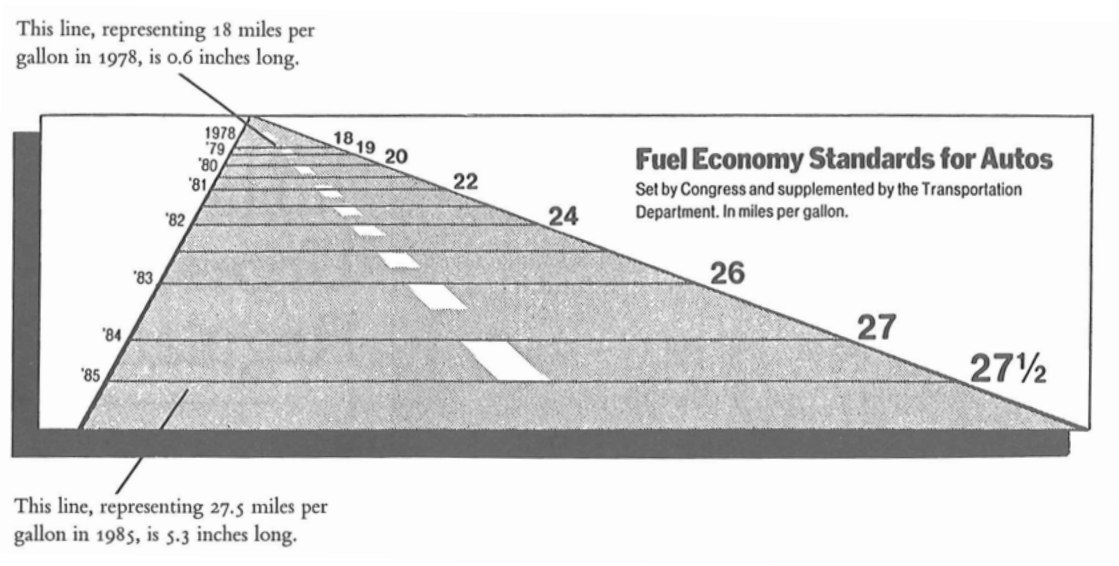
\includegraphics[keepaspectratio]{road.png}}

{[}Tufte, 1991{]} Edward Tufte, The Visual Display of Quantitative
Information, Second Edition, Graphics Press, USA, 1991, p.~57 -- 69.

\[\operatorname{LieFactor} = \frac{\text{size of the effect visible on the chart}}{\text{size of the effect resulting from the data}}\]

\[\text{effect size} = \frac{|\text{second value}-\text{first value}|}{\text{first value}}\]

\pandocbounded{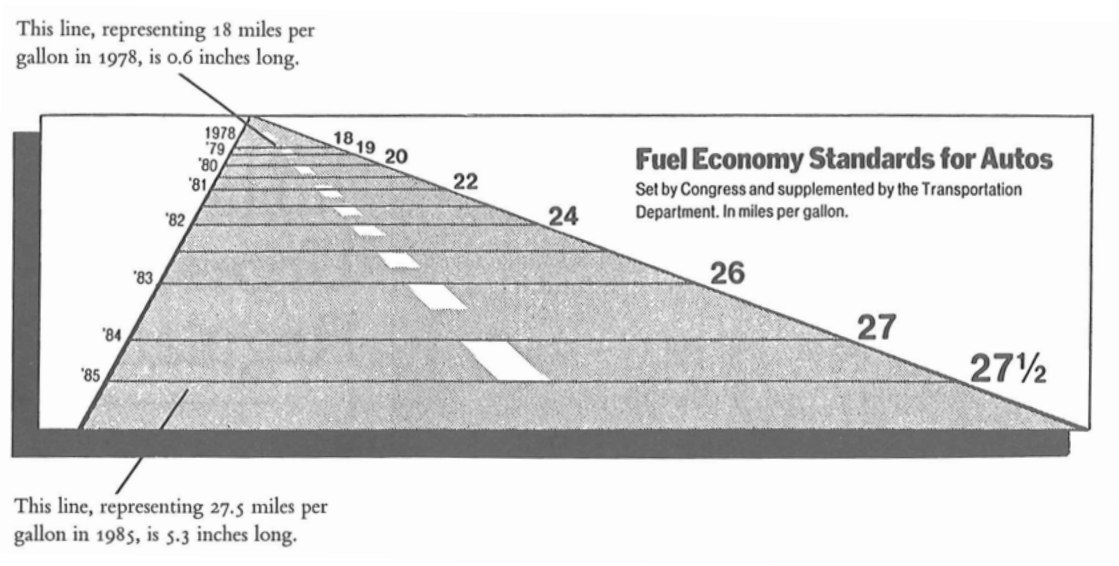
\includegraphics[keepaspectratio]{road.png}}

\[\operatorname{LieFactor} = \frac{\frac{5.3-0.6}{0.6}}{\frac{27.5-18}{18}} \approx 14.8\]

\section{References}\label{references-1}

\begin{itemize}
\tightlist
\item
  https://pl.wikipedia.org/wiki/Wizualizacja
\item
  https://mfiles.pl/pl/index.php/Analiza\_danych, accessed online
  1.04.2019.
\item
  Walesiak M., Gatnar E., Statystyczna analiza danych z wykorzystaniem
  programu R, PWN, Warszawa, 2009.
\item
  Wasilewska E., Statystyka opisowa od podstaw, Podręcznik z zadaniami,
  Wydawnictwo SGGW, Warszawa, 2009.
\item
  https://en.wikipedia.org/wiki/Cognitive\_reflection\_test, accessed
  online 20.03.2023.
\item
  https://qlikblog.pl/edward-tufte-dobre-praktyki-prezentacji-danych/,
  accessed online 20.03.2023.
\end{itemize}

\chapter{Configuration}\label{configuration}

\begin{enumerate}
\def\labelenumi{\arabic{enumi}.}
\tightlist
\item
  In the first step, we create a new project in the chosen location. We
  select venv and one of the Python versions, e.g.~3.13. Finally, click
  the Create button.
\end{enumerate}

\pandocbounded{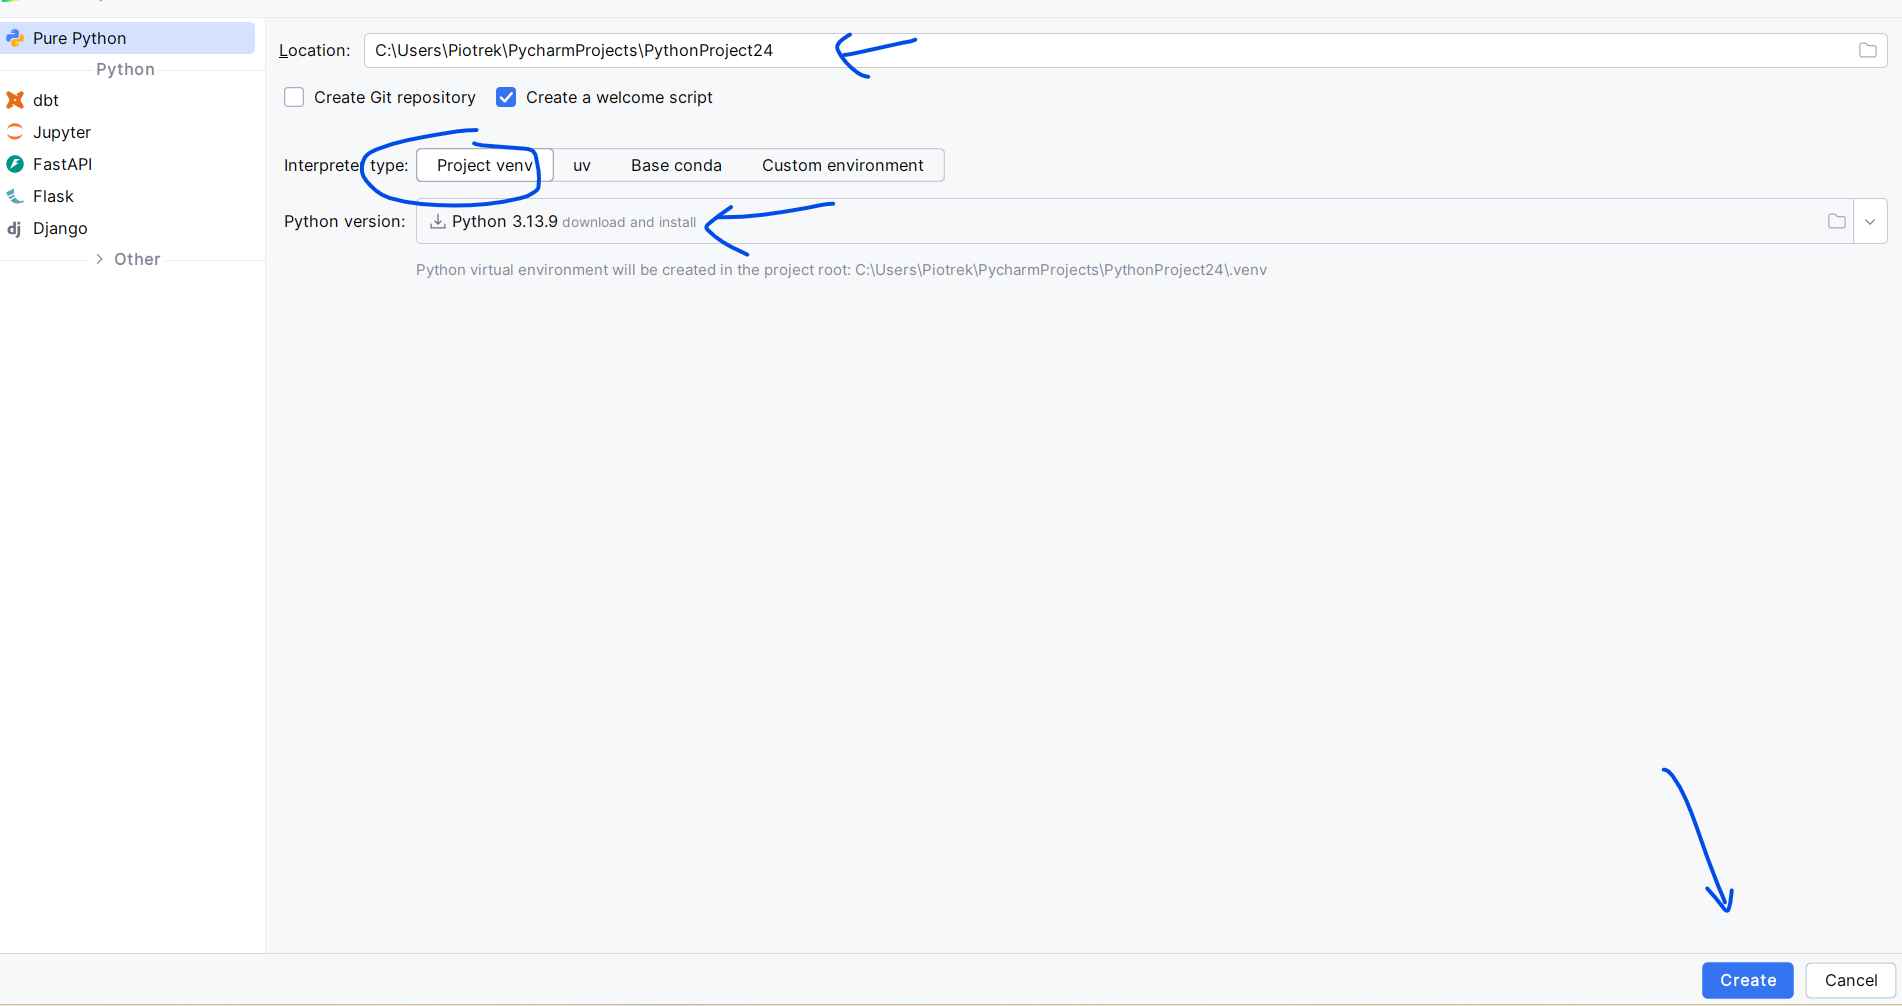
\includegraphics[keepaspectratio]{konf1.png}}

\begin{enumerate}
\def\labelenumi{\arabic{enumi}.}
\setcounter{enumi}{1}
\tightlist
\item
  We add the requirements file
  https://piojas.pl/wp-content/uploads/2026/02/requirements.txt to the
  project's root directory. The file name is important.
\end{enumerate}

\pandocbounded{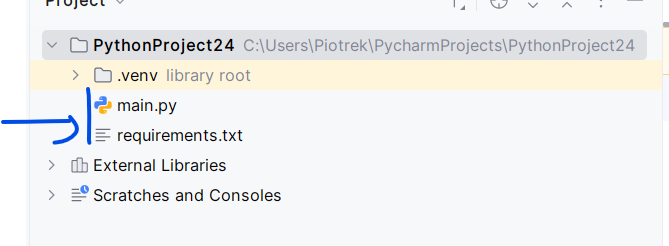
\includegraphics[keepaspectratio]{konf2.png}}

\begin{enumerate}
\def\labelenumi{\arabic{enumi}.}
\setcounter{enumi}{2}
\tightlist
\item
  We open the terminal in PyCharm and type the command:
  \texttt{pip\ install\ -r\ requirements.txt}
\end{enumerate}

\pandocbounded{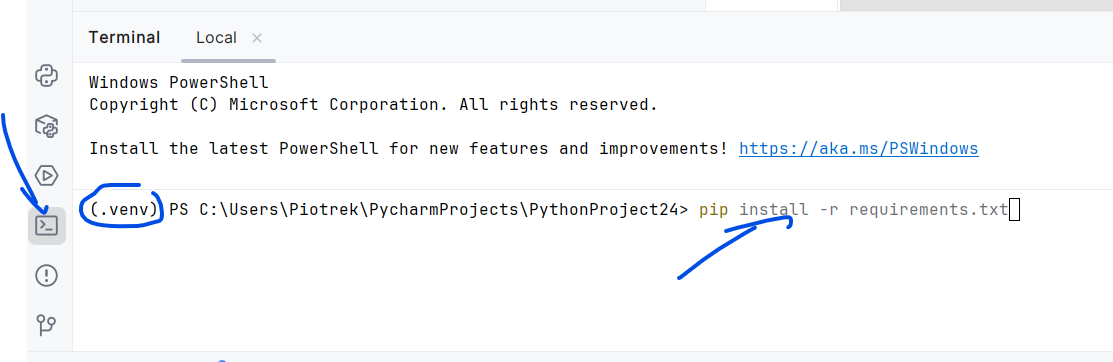
\includegraphics[keepaspectratio]{konf3.png}}

\part{NumPy}

\chapter{NumPy - Getting Started}\label{numpy---getting-started}

NumPy is a Python library for scientific computing.

Applications:

\begin{itemize}
\tightlist
\item
  linear algebra
\item
  advanced mathematical (numerical) computations
\item
  numerical integration
\item
  solving equations
\end{itemize}

\section{Importing the NumPy library}\label{importing-the-numpy-library}

\begin{Shaded}
\begin{Highlighting}[]
\ImportTok{import}\NormalTok{ numpy }\ImportTok{as}\NormalTok{ np}
\end{Highlighting}
\end{Shaded}

The fundamental object in the NumPy library is an N-dimensional array
called \texttt{ndarray}. Each element of the array is treated as a
\texttt{dtype} type.

\begin{Shaded}
\begin{Highlighting}[]
\NormalTok{np.array(}\BuiltInTok{object}\NormalTok{, dtype}\OperatorTok{=}\VariableTok{None}\NormalTok{, }\OperatorTok{*}\NormalTok{, copy}\OperatorTok{=}\VariableTok{True}\NormalTok{, order}\OperatorTok{=}\StringTok{\textquotesingle{}K\textquotesingle{}}\NormalTok{, subok}\OperatorTok{=}\VariableTok{False}\NormalTok{, ndmin}\OperatorTok{=}\DecValTok{0}\NormalTok{, like}\OperatorTok{=}\VariableTok{None}\NormalTok{)}
\end{Highlighting}
\end{Shaded}

\begin{itemize}
\tightlist
\item
  object - an object (or sequence) to be converted into an array
\item
  dtype - type
\item
  copy - whether objects should be copied, default is \texttt{True}
\item
  order - memory layout: C (rows), F (columns), A, K
\item
  subok - handled by subclasses (if \texttt{True}), default is
  \texttt{False}
\item
  ndmin - minimum number of dimensions of the array
\item
  like - creation based on a reference array
\end{itemize}

\protect\phantomsection\label{annotated-cell-3}%
\begin{Shaded}
\begin{Highlighting}[]
\ImportTok{import}\NormalTok{ numpy }\ImportTok{as}\NormalTok{ np}

\NormalTok{a }\OperatorTok{=}\NormalTok{ np.array([}\DecValTok{1}\NormalTok{, }\DecValTok{2}\NormalTok{, }\DecValTok{3}\NormalTok{]) }\hspace*{\fill}\NormalTok{\circled{1}}
\BuiltInTok{print}\NormalTok{(}\StringTok{"a:"}\NormalTok{, a) }
\BuiltInTok{print}\NormalTok{(}\StringTok{"type of a:"}\NormalTok{, }\BuiltInTok{type}\NormalTok{(a)) }\hspace*{\fill}\NormalTok{\circled{2}}
\NormalTok{b }\OperatorTok{=}\NormalTok{ np.array([}\DecValTok{1}\NormalTok{, }\DecValTok{2}\NormalTok{, }\FloatTok{3.0}\NormalTok{]) }\hspace*{\fill}\NormalTok{\circled{3}}
\BuiltInTok{print}\NormalTok{(}\StringTok{"b:"}\NormalTok{, b)}
\NormalTok{c }\OperatorTok{=}\NormalTok{ np.array([[}\DecValTok{1}\NormalTok{, }\DecValTok{2}\NormalTok{], [}\DecValTok{3}\NormalTok{, }\DecValTok{4}\NormalTok{]]) }\hspace*{\fill}\NormalTok{\circled{4}}
\BuiltInTok{print}\NormalTok{(}\StringTok{"c:"}\NormalTok{, c)}
\NormalTok{d }\OperatorTok{=}\NormalTok{ np.array([}\DecValTok{1}\NormalTok{, }\DecValTok{2}\NormalTok{, }\DecValTok{3}\NormalTok{], ndmin}\OperatorTok{=}\DecValTok{2}\NormalTok{) }\hspace*{\fill}\NormalTok{\circled{5}}
\BuiltInTok{print}\NormalTok{(}\StringTok{"d:"}\NormalTok{, d)}
\NormalTok{e }\OperatorTok{=}\NormalTok{ np.array([}\DecValTok{1}\NormalTok{, }\DecValTok{2}\NormalTok{, }\DecValTok{3}\NormalTok{], dtype}\OperatorTok{=}\BuiltInTok{complex}\NormalTok{) }\hspace*{\fill}\NormalTok{\circled{6}}
\BuiltInTok{print}\NormalTok{(}\StringTok{"e:"}\NormalTok{, e)}
\NormalTok{f }\OperatorTok{=}\NormalTok{ np.array(np.asmatrix(}\StringTok{\textquotesingle{}1 2; 3 4\textquotesingle{}}\NormalTok{)) }\hspace*{\fill}\NormalTok{\circled{7}}
\BuiltInTok{print}\NormalTok{(}\StringTok{"f:"}\NormalTok{, f)}
\NormalTok{g }\OperatorTok{=}\NormalTok{ np.array(np.asmatrix(}\StringTok{\textquotesingle{}1 2; 3 4\textquotesingle{}}\NormalTok{), subok}\OperatorTok{=}\VariableTok{True}\NormalTok{) }\hspace*{\fill}\NormalTok{\circled{8}}
\BuiltInTok{print}\NormalTok{(}\StringTok{"g:"}\NormalTok{, g)}
\BuiltInTok{print}\NormalTok{(}\BuiltInTok{type}\NormalTok{(g))}
\end{Highlighting}
\end{Shaded}

\begin{description}
\tightlist
\item[\circled{1}]
Creating an array with default settings.
\item[\circled{2}]
Checking the type.
\item[\circled{3}]
One of the elements is of a different type. Therefore, upcasting to the
``largest'' type occurs.
\item[\circled{4}]
Here we get a 2x2 array.
\item[\circled{5}]
In this line we get an array with dimensions 1x3 (shape
\texttt{(1,\ 3)}).
\item[\circled{6}]
Forcing the \texttt{complex} type --- a type with a wider range.
\item[\circled{7}]
Using the matrix subtype.
\item[\circled{8}]
Preserving the matrix type.
\end{description}

\begin{verbatim}
a: [1 2 3]
type of a: <class 'numpy.ndarray'>
b: [1. 2. 3.]
c: [[1 2]
 [3 4]]
d: [[1 2 3]]
e: [1.+0.j 2.+0.j 3.+0.j]
f: [[1 2]
 [3 4]]
g: [[1 2]
 [3 4]]
<class 'numpy.matrix'>
\end{verbatim}

\chapter{List vs Array}\label{list-vs-array}

\begin{Shaded}
\begin{Highlighting}[]
\ImportTok{import}\NormalTok{ numpy }\ImportTok{as}\NormalTok{ np}
\ImportTok{import}\NormalTok{ time}

\NormalTok{start\_time }\OperatorTok{=}\NormalTok{ time.time()}
\NormalTok{my\_arr }\OperatorTok{=}\NormalTok{ np.arange(}\DecValTok{1000000}\NormalTok{)}
\NormalTok{my\_list }\OperatorTok{=} \BuiltInTok{list}\NormalTok{(}\BuiltInTok{range}\NormalTok{(}\DecValTok{1000000}\NormalTok{))}
\NormalTok{start\_time }\OperatorTok{=}\NormalTok{ time.time()}
\NormalTok{my\_arr2 }\OperatorTok{=}\NormalTok{ my\_arr }\OperatorTok{*} \DecValTok{2}
\BuiltInTok{print}\NormalTok{(}\StringTok{"{-}{-}{-} }\SpecialCharTok{\%s}\StringTok{ seconds {-}{-}{-}"} \OperatorTok{\%}\NormalTok{ (time.time() }\OperatorTok{{-}}\NormalTok{ start\_time))}
\NormalTok{start\_time }\OperatorTok{=}\NormalTok{ time.time()}
\NormalTok{my\_list2 }\OperatorTok{=}\NormalTok{ [x }\OperatorTok{*} \DecValTok{2} \ControlFlowTok{for}\NormalTok{ x }\KeywordTok{in}\NormalTok{ my\_list]}
\BuiltInTok{print}\NormalTok{(}\StringTok{"{-}{-}{-} }\SpecialCharTok{\%s}\StringTok{ seconds {-}{-}{-}"} \OperatorTok{\%}\NormalTok{ (time.time() }\OperatorTok{{-}}\NormalTok{ start\_time))}
\end{Highlighting}
\end{Shaded}

\begin{verbatim}
--- 0.0020012855529785156 seconds ---
--- 0.036900997161865234 seconds ---
\end{verbatim}

\chapter{Array Attributes}\label{array-attributes}

{\def\LTcaptype{none} % do not increment counter
\begin{longtable}[]{@{}
  >{\raggedright\arraybackslash}p{(\linewidth - 2\tabcolsep) * \real{0.5000}}
  >{\raggedright\arraybackslash}p{(\linewidth - 2\tabcolsep) * \real{0.5000}}@{}}
\toprule\noalign{}
\begin{minipage}[b]{\linewidth}\raggedright
Attribute
\end{minipage} & \begin{minipage}[b]{\linewidth}\raggedright
Description
\end{minipage} \\
\midrule\noalign{}
\endhead
\bottomrule\noalign{}
\endlastfoot
\texttt{shape} & tuple with information about the number of elements for
each dimension \\
\texttt{size} & total number of elements in the array \\
\texttt{ndim} & number of dimensions of the array \\
\texttt{nbytes} & number of bytes the array occupies in memory \\
\texttt{dtype} & data type stored in the array (e.g.~\texttt{int64},
\texttt{float64}) \\
\end{longtable}
}

\begin{Shaded}
\begin{Highlighting}[]
\ImportTok{import}\NormalTok{ numpy }\ImportTok{as}\NormalTok{ np}

\NormalTok{tab1 }\OperatorTok{=}\NormalTok{ np.array([}\DecValTok{2}\NormalTok{, }\OperatorTok{{-}}\DecValTok{3}\NormalTok{, }\DecValTok{4}\NormalTok{, }\OperatorTok{{-}}\DecValTok{8}\NormalTok{, }\DecValTok{1}\NormalTok{])}
\BuiltInTok{print}\NormalTok{(}\StringTok{"type:"}\NormalTok{, }\BuiltInTok{type}\NormalTok{(tab1))}
\BuiltInTok{print}\NormalTok{(}\StringTok{"shape:"}\NormalTok{, tab1.shape)}
\BuiltInTok{print}\NormalTok{(}\StringTok{"size:"}\NormalTok{, tab1.size)}
\BuiltInTok{print}\NormalTok{(}\StringTok{"ndim:"}\NormalTok{, tab1.ndim)}
\BuiltInTok{print}\NormalTok{(}\StringTok{"nbytes:"}\NormalTok{, tab1.nbytes)}
\BuiltInTok{print}\NormalTok{(}\StringTok{"dtype:"}\NormalTok{, tab1.dtype)}
\end{Highlighting}
\end{Shaded}

\begin{verbatim}
type: <class 'numpy.ndarray'>
shape: (5,)
size: 5
ndim: 1
nbytes: 40
dtype: int64
\end{verbatim}

\begin{Shaded}
\begin{Highlighting}[]
\ImportTok{import}\NormalTok{ numpy }\ImportTok{as}\NormalTok{ np}

\NormalTok{tab2 }\OperatorTok{=}\NormalTok{ np.array([[}\DecValTok{2}\NormalTok{, }\OperatorTok{{-}}\DecValTok{3}\NormalTok{], [}\DecValTok{4}\NormalTok{, }\OperatorTok{{-}}\DecValTok{8}\NormalTok{]])}
\BuiltInTok{print}\NormalTok{(}\StringTok{"type:"}\NormalTok{, }\BuiltInTok{type}\NormalTok{(tab2))}
\BuiltInTok{print}\NormalTok{(}\StringTok{"shape:"}\NormalTok{, tab2.shape)}
\BuiltInTok{print}\NormalTok{(}\StringTok{"size:"}\NormalTok{, tab2.size)}
\BuiltInTok{print}\NormalTok{(}\StringTok{"ndim:"}\NormalTok{, tab2.ndim)}
\BuiltInTok{print}\NormalTok{(}\StringTok{"nbytes:"}\NormalTok{, tab2.nbytes)}
\BuiltInTok{print}\NormalTok{(}\StringTok{"dtype:"}\NormalTok{, tab2.dtype)}
\end{Highlighting}
\end{Shaded}

\begin{verbatim}
type: <class 'numpy.ndarray'>
shape: (2, 2)
size: 4
ndim: 2
nbytes: 32
dtype: int64
\end{verbatim}

NumPy does not support ragged arrays. The following code will produce an
error:

\begin{Shaded}
\begin{Highlighting}[]
\ImportTok{import}\NormalTok{ numpy }\ImportTok{as}\NormalTok{ np}

\NormalTok{tab3 }\OperatorTok{=}\NormalTok{ np.array([[}\DecValTok{2}\NormalTok{, }\OperatorTok{{-}}\DecValTok{3}\NormalTok{], [}\DecValTok{4}\NormalTok{, }\OperatorTok{{-}}\DecValTok{8}\NormalTok{, }\DecValTok{5}\NormalTok{], [}\DecValTok{3}\NormalTok{]])}
\end{Highlighting}
\end{Shaded}

\chapter{Data Types}\label{data-types}

{\def\LTcaptype{none} % do not increment counter
\begin{longtable}[]{@{}
  >{\raggedright\arraybackslash}p{(\linewidth - 2\tabcolsep) * \real{0.5000}}
  >{\raggedright\arraybackslash}p{(\linewidth - 2\tabcolsep) * \real{0.5000}}@{}}
\toprule\noalign{}
\endhead
\bottomrule\noalign{}
\endlastfoot
Integer types &
\texttt{int},\texttt{int8},\texttt{int16},\texttt{int32},\texttt{int64} \\
Unsigned integer types &
\texttt{uint},\texttt{uint8},\texttt{uint16},\texttt{uint32},\texttt{uint64} \\
Boolean type & \texttt{bool} \\
Floating-point types & \texttt{float}, \texttt{float16},
\texttt{float32}, \texttt{float64}, \texttt{float128} \\
Complex floating-point types & \texttt{complex}, \texttt{complex64},
\texttt{complex128}, \texttt{complex256} \\
String & \texttt{str} \\
\end{longtable}
}

\begin{Shaded}
\begin{Highlighting}[]
\ImportTok{import}\NormalTok{ numpy }\ImportTok{as}\NormalTok{ np}

\NormalTok{tab }\OperatorTok{=}\NormalTok{ np.array([[}\DecValTok{2}\NormalTok{, }\OperatorTok{{-}}\DecValTok{3}\NormalTok{], [}\DecValTok{4}\NormalTok{, }\OperatorTok{{-}}\DecValTok{8}\NormalTok{]])}
\BuiltInTok{print}\NormalTok{(tab)}
\NormalTok{tab2 }\OperatorTok{=}\NormalTok{ np.array([[}\DecValTok{2}\NormalTok{, }\OperatorTok{{-}}\DecValTok{3}\NormalTok{], [}\DecValTok{4}\NormalTok{, }\OperatorTok{{-}}\DecValTok{8}\NormalTok{]], dtype}\OperatorTok{=}\BuiltInTok{int}\NormalTok{)}
\BuiltInTok{print}\NormalTok{(tab2)}
\NormalTok{tab3 }\OperatorTok{=}\NormalTok{ np.array([[}\DecValTok{2}\NormalTok{, }\OperatorTok{{-}}\DecValTok{3}\NormalTok{], [}\DecValTok{4}\NormalTok{, }\OperatorTok{{-}}\DecValTok{8}\NormalTok{]], dtype}\OperatorTok{=}\BuiltInTok{float}\NormalTok{)}
\BuiltInTok{print}\NormalTok{(tab3)}
\NormalTok{tab4 }\OperatorTok{=}\NormalTok{ np.array([[}\DecValTok{2}\NormalTok{, }\OperatorTok{{-}}\DecValTok{3}\NormalTok{], [}\DecValTok{4}\NormalTok{, }\OperatorTok{{-}}\DecValTok{8}\NormalTok{]], dtype}\OperatorTok{=}\BuiltInTok{complex}\NormalTok{)}
\BuiltInTok{print}\NormalTok{(tab4)}
\end{Highlighting}
\end{Shaded}

\begin{verbatim}
[[ 2 -3]
 [ 4 -8]]
[[ 2 -3]
 [ 4 -8]]
[[ 2. -3.]
 [ 4. -8.]]
[[ 2.+0.j -3.+0.j]
 [ 4.+0.j -8.+0.j]]
\end{verbatim}

\chapter{Creating Arrays}\label{creating-arrays}

\texttt{np.array} - arguments are cast to an array (anything iterable) -
it's worth checking the size/shape

\begin{Shaded}
\begin{Highlighting}[]
\ImportTok{import}\NormalTok{ numpy }\ImportTok{as}\NormalTok{ np}

\NormalTok{tab }\OperatorTok{=}\NormalTok{ np.array([}\DecValTok{2}\NormalTok{, }\OperatorTok{{-}}\DecValTok{3}\NormalTok{, }\DecValTok{4}\NormalTok{])}
\BuiltInTok{print}\NormalTok{(tab)}
\BuiltInTok{print}\NormalTok{(}\StringTok{"size:"}\NormalTok{, tab.size)}
\NormalTok{tab2 }\OperatorTok{=}\NormalTok{ np.array((}\DecValTok{4}\NormalTok{, }\OperatorTok{{-}}\DecValTok{3}\NormalTok{, }\DecValTok{3}\NormalTok{, }\DecValTok{2}\NormalTok{))}
\BuiltInTok{print}\NormalTok{(tab2)}
\BuiltInTok{print}\NormalTok{(}\StringTok{"size:"}\NormalTok{, tab2.size)}
\NormalTok{tab3 }\OperatorTok{=}\NormalTok{ np.array(\{}\DecValTok{3}\NormalTok{, }\DecValTok{3}\NormalTok{, }\DecValTok{2}\NormalTok{, }\DecValTok{5}\NormalTok{, }\DecValTok{2}\NormalTok{\})}
\BuiltInTok{print}\NormalTok{(tab3)}
\BuiltInTok{print}\NormalTok{(}\StringTok{"size:"}\NormalTok{, tab3.size)}
\NormalTok{tab4 }\OperatorTok{=}\NormalTok{ np.array(\{}\StringTok{"pl"}\NormalTok{: }\DecValTok{344}\NormalTok{, }\StringTok{"en"}\NormalTok{: }\DecValTok{22}\NormalTok{\})}
\BuiltInTok{print}\NormalTok{(tab4)}
\BuiltInTok{print}\NormalTok{(}\StringTok{"size:"}\NormalTok{, tab4.size)}
\end{Highlighting}
\end{Shaded}

\begin{verbatim}
[ 2 -3  4]
size: 3
[ 4 -3  3  2]
size: 4
{2, 3, 5}
size: 1
{'pl': 344, 'en': 22}
size: 1
\end{verbatim}

\texttt{np.zeros} - creates an array filled with zeros

\begin{Shaded}
\begin{Highlighting}[]
\ImportTok{import}\NormalTok{ numpy }\ImportTok{as}\NormalTok{ np}

\NormalTok{tab }\OperatorTok{=}\NormalTok{ np.zeros(}\DecValTok{4}\NormalTok{)}
\BuiltInTok{print}\NormalTok{(tab)}
\BuiltInTok{print}\NormalTok{(tab.shape)}
\NormalTok{tab2 }\OperatorTok{=}\NormalTok{ np.zeros([}\DecValTok{2}\NormalTok{, }\DecValTok{3}\NormalTok{])}
\BuiltInTok{print}\NormalTok{(tab2)}
\BuiltInTok{print}\NormalTok{(tab2.shape)}
\NormalTok{tab3 }\OperatorTok{=}\NormalTok{ np.zeros([}\DecValTok{2}\NormalTok{, }\DecValTok{3}\NormalTok{, }\DecValTok{4}\NormalTok{])}
\BuiltInTok{print}\NormalTok{(tab3)}
\BuiltInTok{print}\NormalTok{(tab3.shape)}
\end{Highlighting}
\end{Shaded}

\begin{verbatim}
[0. 0. 0. 0.]
(4,)
[[0. 0. 0.]
 [0. 0. 0.]]
(2, 3)
[[[0. 0. 0. 0.]
  [0. 0. 0. 0.]
  [0. 0. 0. 0.]]

 [[0. 0. 0. 0.]
  [0. 0. 0. 0.]
  [0. 0. 0. 0.]]]
(2, 3, 4)
\end{verbatim}

\texttt{np.ones} - creates an array filled with ones (this is not the
equivalent of an identity matrix!)

\begin{Shaded}
\begin{Highlighting}[]
\ImportTok{import}\NormalTok{ numpy }\ImportTok{as}\NormalTok{ np}

\NormalTok{tab }\OperatorTok{=}\NormalTok{ np.ones(}\DecValTok{4}\NormalTok{)}
\BuiltInTok{print}\NormalTok{(tab)}
\BuiltInTok{print}\NormalTok{(tab.shape)}
\NormalTok{tab2 }\OperatorTok{=}\NormalTok{ np.ones([}\DecValTok{2}\NormalTok{, }\DecValTok{3}\NormalTok{])}
\BuiltInTok{print}\NormalTok{(tab2)}
\BuiltInTok{print}\NormalTok{(tab2.shape)}
\NormalTok{tab3 }\OperatorTok{=}\NormalTok{ np.ones([}\DecValTok{2}\NormalTok{, }\DecValTok{3}\NormalTok{, }\DecValTok{4}\NormalTok{])}
\BuiltInTok{print}\NormalTok{(tab3)}
\BuiltInTok{print}\NormalTok{(tab3.shape)}
\end{Highlighting}
\end{Shaded}

\begin{verbatim}
[1. 1. 1. 1.]
(4,)
[[1. 1. 1.]
 [1. 1. 1.]]
(2, 3)
[[[1. 1. 1. 1.]
  [1. 1. 1. 1.]
  [1. 1. 1. 1.]]

 [[1. 1. 1. 1.]
  [1. 1. 1. 1.]
  [1. 1. 1. 1.]]]
(2, 3, 4)
\end{verbatim}

\texttt{np.diag} - creates an array corresponding to a diagonal matrix

\begin{Shaded}
\begin{Highlighting}[]
\ImportTok{import}\NormalTok{ numpy }\ImportTok{as}\NormalTok{ np}

\BuiltInTok{print}\NormalTok{(}\StringTok{"tab0"}\NormalTok{)}
\NormalTok{tab0 }\OperatorTok{=}\NormalTok{ np.diag([}\DecValTok{3}\NormalTok{, }\DecValTok{4}\NormalTok{, }\DecValTok{5}\NormalTok{])}
\BuiltInTok{print}\NormalTok{(tab0)}
\BuiltInTok{print}\NormalTok{(}\StringTok{"tab1"}\NormalTok{)}
\NormalTok{tab1 }\OperatorTok{=}\NormalTok{ np.array([[}\DecValTok{2}\NormalTok{, }\DecValTok{3}\NormalTok{, }\DecValTok{4}\NormalTok{], [}\DecValTok{3}\NormalTok{, }\OperatorTok{{-}}\DecValTok{4}\NormalTok{, }\DecValTok{5}\NormalTok{], [}\DecValTok{3}\NormalTok{, }\DecValTok{4}\NormalTok{, }\OperatorTok{{-}}\DecValTok{5}\NormalTok{]])}
\BuiltInTok{print}\NormalTok{(tab1)}
\NormalTok{tab2 }\OperatorTok{=}\NormalTok{ np.diag(tab1)}
\BuiltInTok{print}\NormalTok{(}\StringTok{"tab2"}\NormalTok{)}
\BuiltInTok{print}\NormalTok{(tab2)}
\NormalTok{tab3 }\OperatorTok{=}\NormalTok{ np.diag(tab1, k}\OperatorTok{=}\DecValTok{1}\NormalTok{)}
\BuiltInTok{print}\NormalTok{(}\StringTok{"tab3"}\NormalTok{)}
\BuiltInTok{print}\NormalTok{(tab3)}
\BuiltInTok{print}\NormalTok{(}\StringTok{"tab4"}\NormalTok{)}
\NormalTok{tab4 }\OperatorTok{=}\NormalTok{ np.diag(tab1, k}\OperatorTok{={-}}\DecValTok{2}\NormalTok{)}
\BuiltInTok{print}\NormalTok{(tab4)}
\BuiltInTok{print}\NormalTok{(}\StringTok{"tab5"}\NormalTok{)}
\NormalTok{tab5 }\OperatorTok{=}\NormalTok{ np.diag(np.diag(tab1))}
\BuiltInTok{print}\NormalTok{(tab5)}
\end{Highlighting}
\end{Shaded}

\begin{verbatim}
tab0
[[3 0 0]
 [0 4 0]
 [0 0 5]]
tab1
[[ 2  3  4]
 [ 3 -4  5]
 [ 3  4 -5]]
tab2
[ 2 -4 -5]
tab3
[3 5]
tab4
[3]
tab5
[[ 2  0  0]
 [ 0 -4  0]
 [ 0  0 -5]]
\end{verbatim}

\texttt{np.arange} - array filled with evenly spaced values

Syntax:
\texttt{numpy.arange({[}start,\ {]}stop,\ {[}step,\ {]}dtype=None)}

Works similarly to the \texttt{range} function, but allows fractional
numbers.

\begin{Shaded}
\begin{Highlighting}[]
\ImportTok{import}\NormalTok{ numpy }\ImportTok{as}\NormalTok{ np}

\NormalTok{a }\OperatorTok{=}\NormalTok{ np.arange(}\DecValTok{3}\NormalTok{)}
\BuiltInTok{print}\NormalTok{(a)}
\NormalTok{b }\OperatorTok{=}\NormalTok{ np.arange(}\FloatTok{3.0}\NormalTok{)}
\BuiltInTok{print}\NormalTok{(b)}
\NormalTok{c }\OperatorTok{=}\NormalTok{ np.arange(}\DecValTok{3}\NormalTok{, }\DecValTok{7}\NormalTok{)}
\BuiltInTok{print}\NormalTok{(c)}
\NormalTok{d }\OperatorTok{=}\NormalTok{ np.arange(}\DecValTok{3}\NormalTok{, }\DecValTok{11}\NormalTok{, }\DecValTok{2}\NormalTok{)}
\BuiltInTok{print}\NormalTok{(d)}
\NormalTok{e }\OperatorTok{=}\NormalTok{ np.arange(}\DecValTok{0}\NormalTok{, }\DecValTok{1}\NormalTok{, }\FloatTok{0.1}\NormalTok{)}
\BuiltInTok{print}\NormalTok{(e)}
\NormalTok{f }\OperatorTok{=}\NormalTok{ np.arange(}\DecValTok{3}\NormalTok{, }\DecValTok{11}\NormalTok{, }\DecValTok{2}\NormalTok{, dtype}\OperatorTok{=}\BuiltInTok{float}\NormalTok{)}
\BuiltInTok{print}\NormalTok{(f)}
\NormalTok{g }\OperatorTok{=}\NormalTok{ np.arange(}\DecValTok{3}\NormalTok{, }\DecValTok{10}\NormalTok{, }\DecValTok{2}\NormalTok{)}
\BuiltInTok{print}\NormalTok{(g)}
\end{Highlighting}
\end{Shaded}

\begin{verbatim}
[0 1 2]
[0. 1. 2.]
[3 4 5 6]
[3 5 7 9]
[0.  0.1 0.2 0.3 0.4 0.5 0.6 0.7 0.8 0.9]
[3. 5. 7. 9.]
[3 5 7 9]
\end{verbatim}

\texttt{np.linspace} - array filled with evenly spaced values on a
linear scale

\texttt{np.linspace(start,\ stop,\ num)} generates an array of evenly
spaced values. For example, \texttt{np.linspace(2.0,\ 3.0,\ num=5)}
produces \texttt{2,\ 2.25,\ 2.5,\ 2.75,\ 3} --- the interval is divided
into \texttt{num\ -\ 1} equal parts. Setting \texttt{endpoint=False}
removes the last point (from the right side), and the interval is then
divided into \texttt{num} equal parts instead. The \texttt{dtype}
parameter forces the output type --- typically set to \texttt{int}, in
which case the results may have the fractional part truncated.

\begin{Shaded}
\begin{Highlighting}[]
\ImportTok{import}\NormalTok{ numpy }\ImportTok{as}\NormalTok{ np}

\NormalTok{a }\OperatorTok{=}\NormalTok{ np.linspace(}\FloatTok{2.0}\NormalTok{, }\FloatTok{3.0}\NormalTok{, num}\OperatorTok{=}\DecValTok{5}\NormalTok{)}
\BuiltInTok{print}\NormalTok{(a)}
\NormalTok{b }\OperatorTok{=}\NormalTok{ np.linspace(}\FloatTok{2.0}\NormalTok{, }\FloatTok{3.0}\NormalTok{, num}\OperatorTok{=}\DecValTok{5}\NormalTok{, endpoint}\OperatorTok{=}\VariableTok{False}\NormalTok{)}
\BuiltInTok{print}\NormalTok{(b)}
\NormalTok{c }\OperatorTok{=}\NormalTok{ np.linspace(}\DecValTok{10}\NormalTok{, }\DecValTok{20}\NormalTok{, num}\OperatorTok{=}\DecValTok{4}\NormalTok{)}
\BuiltInTok{print}\NormalTok{(c)}
\NormalTok{d }\OperatorTok{=}\NormalTok{ np.linspace(}\DecValTok{10}\NormalTok{, }\DecValTok{20}\NormalTok{, num}\OperatorTok{=}\DecValTok{4}\NormalTok{, dtype}\OperatorTok{=}\BuiltInTok{int}\NormalTok{)}
\BuiltInTok{print}\NormalTok{(d)}
\end{Highlighting}
\end{Shaded}

\begin{verbatim}
[2.   2.25 2.5  2.75 3.  ]
[2.  2.2 2.4 2.6 2.8]
[10.         13.33333333 16.66666667 20.        ]
[10 13 16 20]
\end{verbatim}

\texttt{np.logspace} - array filled with values on a logarithmic scale

Syntax:
\texttt{numpy.logspace(start,\ stop,\ num=50,\ endpoint=True,\ base=10.0,\ dtype=None,\ axis=0)}

The function \texttt{np.logspace(2.0,\ 3.0,\ num=4)} generates 4 numbers
spaced evenly on a logarithmic scale between 10\^{}2 and 10\^{}3. The
default base is 10. First, the exponents are computed as equally spaced
points in the interval {[}2.0, 3.0{]}, which gives approximately 2,
2.33, 2.66, and 3.0. Then each exponent is used as the power of 10,
producing the output values 10\^{}2 = 100, 10\^{}2.33 ≈ 215.44,
10\^{}2.66 ≈ 464.16, and 10\^{}3 = 1000. An important consequence is
that while the exponents are uniformly distributed, the resulting values
are not --- the distances between consecutive output numbers grow larger
as the values increase. This is the key distinction between
\texttt{np.logspace} and \texttt{np.linspace}: the former creates equal
spacing in log-scale (i.e.~between the exponents), not in the actual
output values.

\begin{Shaded}
\begin{Highlighting}[]
\ImportTok{import}\NormalTok{ numpy }\ImportTok{as}\NormalTok{ np}

\NormalTok{a }\OperatorTok{=}\NormalTok{ np.logspace(}\FloatTok{2.0}\NormalTok{, }\FloatTok{3.0}\NormalTok{, num}\OperatorTok{=}\DecValTok{4}\NormalTok{)}
\BuiltInTok{print}\NormalTok{(a)}
\NormalTok{b }\OperatorTok{=}\NormalTok{ np.logspace(}\FloatTok{2.0}\NormalTok{, }\FloatTok{3.0}\NormalTok{, num}\OperatorTok{=}\DecValTok{4}\NormalTok{, endpoint}\OperatorTok{=}\VariableTok{False}\NormalTok{)}
\BuiltInTok{print}\NormalTok{(b)}
\NormalTok{c }\OperatorTok{=}\NormalTok{ np.logspace(}\FloatTok{2.0}\NormalTok{, }\FloatTok{3.0}\NormalTok{, num}\OperatorTok{=}\DecValTok{4}\NormalTok{, base}\OperatorTok{=}\FloatTok{2.0}\NormalTok{)}
\BuiltInTok{print}\NormalTok{(c)}
\end{Highlighting}
\end{Shaded}

\begin{verbatim}
[ 100.          215.443469    464.15888336 1000.        ]
[100.         177.827941   316.22776602 562.34132519]
[4.         5.0396842  6.34960421 8.        ]
\end{verbatim}

\texttt{np.empty} - empty (uninitialized) array - specific values are
not ``guaranteed''

\begin{Shaded}
\begin{Highlighting}[]
\ImportTok{import}\NormalTok{ numpy }\ImportTok{as}\NormalTok{ np}

\NormalTok{a }\OperatorTok{=}\NormalTok{ np.empty(}\DecValTok{3}\NormalTok{)}
\BuiltInTok{print}\NormalTok{(a)}
\NormalTok{b }\OperatorTok{=}\NormalTok{ np.empty(}\DecValTok{3}\NormalTok{, dtype}\OperatorTok{=}\BuiltInTok{int}\NormalTok{)}
\BuiltInTok{print}\NormalTok{(b)}
\end{Highlighting}
\end{Shaded}

\begin{verbatim}
[0. 1. 2.]
[                  0 4607182418800017408 4611686018427387904]
\end{verbatim}

\texttt{np.identity} - array resembling an identity matrix

\texttt{np.eye} - array with ones on the diagonal (remaining values are
zeros)

\begin{Shaded}
\begin{Highlighting}[]
\ImportTok{import}\NormalTok{ numpy }\ImportTok{as}\NormalTok{ np}

\BuiltInTok{print}\NormalTok{(}\StringTok{"a"}\NormalTok{)}
\NormalTok{a }\OperatorTok{=}\NormalTok{ np.identity(}\DecValTok{4}\NormalTok{)}
\BuiltInTok{print}\NormalTok{(a)}
\BuiltInTok{print}\NormalTok{(}\StringTok{"b"}\NormalTok{)}
\NormalTok{b }\OperatorTok{=}\NormalTok{ np.eye(}\DecValTok{4}\NormalTok{, k}\OperatorTok{=}\DecValTok{1}\NormalTok{)}
\BuiltInTok{print}\NormalTok{(b)}
\BuiltInTok{print}\NormalTok{(}\StringTok{"c"}\NormalTok{)}
\NormalTok{c }\OperatorTok{=}\NormalTok{ np.eye(}\DecValTok{4}\NormalTok{, k}\OperatorTok{=}\DecValTok{2}\NormalTok{)}
\BuiltInTok{print}\NormalTok{(c)}
\BuiltInTok{print}\NormalTok{(}\StringTok{"d"}\NormalTok{)}
\NormalTok{d }\OperatorTok{=}\NormalTok{ np.eye(}\DecValTok{4}\NormalTok{, k}\OperatorTok{={-}}\DecValTok{1}\NormalTok{)}
\BuiltInTok{print}\NormalTok{(d)}
\end{Highlighting}
\end{Shaded}

\begin{verbatim}
a
[[1. 0. 0. 0.]
 [0. 1. 0. 0.]
 [0. 0. 1. 0.]
 [0. 0. 0. 1.]]
b
[[0. 1. 0. 0.]
 [0. 0. 1. 0.]
 [0. 0. 0. 1.]
 [0. 0. 0. 0.]]
c
[[0. 0. 1. 0.]
 [0. 0. 0. 1.]
 [0. 0. 0. 0.]
 [0. 0. 0. 0.]]
d
[[0. 0. 0. 0.]
 [1. 0. 0. 0.]
 [0. 1. 0. 0.]
 [0. 0. 1. 0.]]
\end{verbatim}




\end{document}
